\documentclass[10pt]{article}
% DRAFT in TMLR style as a stand-in. BEFORE submitting to the NeurIPS ICBINB-bio workshop,
% replace with the official neurips_20XX.sty from that year's call (the layout/anonymity rules
% are mandated by the workshop). Content and length (4 pages + refs) are workshop-ready.
\usepackage{tmlr}

\usepackage{booktabs}
\usepackage{amsmath}
\usepackage{graphicx}
\usepackage{hyperref}
\usepackage{url}

\title{Where a Mind-Migration Pipeline Breaks: A Functional-Preservation Audit\\
of Partition, Transport, and Local-Rule Writing}

\author{\name Anonymous \email anon@example.com \\ \addr Anonymous Institution}
\def\month{11}\def\year{2026}
\def\openreview{\url{https://openreview.net/forum?id=XXXXXXXX}}

\begin{document}
\maketitle

\begin{abstract}
Speculative ``mind-migration'' pipelines propose partitioning a brain into a regenerable Base-OS
and a transferable identity payload, compressing the payload, aligning it to a new substrate, and
writing it in with local plasticity. We ask whether each stage is coherent in simulation, using a
Functional Preservation Score (FPS) --- a null-normalised measure of how much input--output
function survives an operation --- on the \emph{C. elegans} connectome and small recurrent
networks that run on a laptop. All three migration stages fail, for largely independent reasons:
the identity payload is not a functionally separable module ($p\geq0.16$); Gromov--Wasserstein
transport collapses once the target's real wiring is respected (fidelity $1.00\!\to\!0.40$,
$p<10^{-3}$) or alignment is imperfect ($0.06$); and biologically plausible local plasticity
cannot reach the function the target topology provably admits (gap $0.45$, $p<10^{-3}$, $d=2.0$),
with sleep-ripple timing providing no benefit. The common obstacle is the target substrate's own
wiring. We frame this as a reusable recipe --- make preservation measurable, verify the metric has
headroom over a trivial null, and test each pipeline stage against an achievable upper bound ---
for failure analysis of ambitious biological-ML pipelines.
\end{abstract}

\section{Motivation}
Ambitious biological-ML pipelines are often argued as compositions of individually plausible
steps. Mind migration is an extreme case: each step borrows a real result, but the composition is
untested and several steps have no evidence at any scale. We take the computational core and ask a
single measurable question per stage --- does it preserve function? --- and report where it breaks.
This short paper focuses on the negative result (the three-stage pipeline); the companion work
also characterises connectome and replay compression, which succeed.

\section{Method: FPS and the audit protocol}
For a reference system with outputs $Y_{\mathrm{ref}}$ and a transformed system with outputs $Y$,
let $\mathrm{raw}(Y)=1-\lVert Y-Y_{\mathrm{ref}}\rVert^2/\lVert Y_{\mathrm{ref}}-\overline{Y_{\mathrm{ref}}}\rVert^2$,
and normalise by the best trivial baseline $Y_{\mathrm{null}}$ (shuffle or predict-the-mean):
$\mathrm{FPS}=\mathrm{clip}((\mathrm{raw}(Y)-\mathrm{raw}(Y_{\mathrm{null}}))/(1-\mathrm{raw}(Y_{\mathrm{null}})),0,1)$.
The protocol has three rules learned the hard way: validate on real data; verify the metric beats
its trivial null \emph{before} trusting a comparison; and compare each stage to an achievable
upper bound, not to perfection. Numbers are reported with bootstrap 95\% CIs and permutation
$p$-values.

\section{Result: the pipeline breaks at every stage}
\textbf{Partition is not separable.} Holding the sensory/motor interface fixed, ablating the
asserted interneuron ``payload'' of the real \emph{C. elegans} connectome is no more disruptive
than ablating a random interneuron subset of the same size ($p=0.17,0.16,0.27,0.37$ across payload
fractions $0.1$--$0.4$; 500-sample null). Function is distributed; there is no module to lift out.

\textbf{Transport breaks under realism} (Figure~\ref{fig:w}, left). Entropic Gromov--Wasserstein
recovers $0.76$ of a ground-truth correspondence at $5\%$ divergence, but transporting weights to a
second individual preserves function only in a doubly idealised limit. With an oracle
correspondence and unconstrained writing, fidelity is $1.00$; once the target's wiring is respected
it falls to $0.40$ (95\% CI $[0.31,0.49]$, $p=3\times10^{-4}$), and with the estimated
correspondence to $0.06$ ($p=2\times10^{-4}$).

\textbf{Local-rule writing cannot reach the target} (Figure~\ref{fig:w}, right). A global optimiser
installs the target function on the fixed topology (ceiling $1.00$), but strictly local
reward-modulated plasticity reaches only $0.55$ ($[0.36,0.73]$), a plausibility gap of $0.45$
($[0.27,0.64]$, $p=10^{-4}$, $d=2.0$). Sleep-ripple-timed gating confers no advantage.

The three failures are independent and compound, and the target substrate's own wiring is the
binding limit shared by transport and writing --- the constraint the original proposal assumes away.

\begin{figure}[t]
\centering
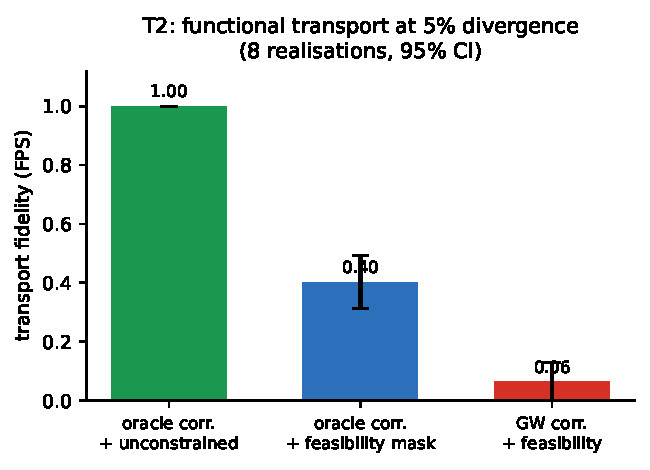
\includegraphics[width=0.46\linewidth]{figures/fig3_t2_transport.pdf}\hfill
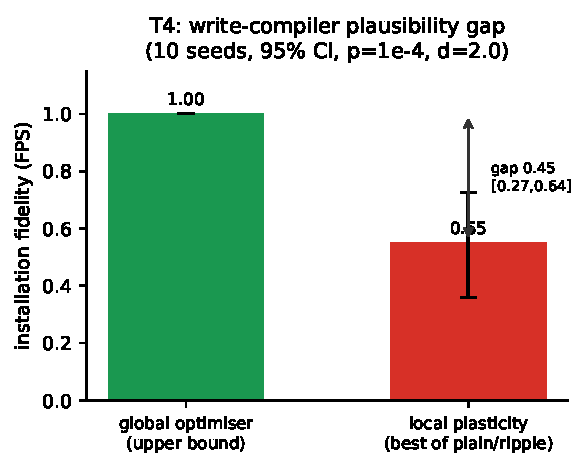
\includegraphics[width=0.46\linewidth]{figures/fig4_t4_gap.pdf}
\caption{Left: transport fidelity at $5\%$ divergence collapses under the feasibility mask and
under estimated alignment (95\% CI). Right: local plasticity cannot close the gap to the global
ceiling the topology admits.}
\label{fig:w}
\end{figure}

\section{Takeaway}
The pipeline is not merely unbuilt; its middle stages are incoherent in simulation on the nearest
testable substrate, each for a different reason. More useful than the specific negative is the
recipe: a measurable preservation score, a trivial-null headroom check, and an achievable upper
bound per stage turn an unfalsifiable roadmap into a set of falsifiable claims. Scope: nematode and
small-network scale; nothing here concerns reading or writing a living brain.

\bibliographystyle{tmlr}
\bibliography{references}
\end{document}
